% Control case for the Polynomial-PEPS figure: the author's own \geometryrow/\geometryband macros
% drawn for real, and the same coordinates probed. The picture's axes are x=.86cm,y=1cm, so a
% probe is the only way to see whether the canvas numbers carry the .86 and the pgfmath midpoint.
\documentclass{article}
\usepackage{tikz}
\usetikzlibrary{arrows.meta,calc,patterns,positioning,decorations.pathreplacing}
\pagestyle{empty}
\makeatletter
% \pgfpointxy answers in the current frame; \pgfpointtransformed is what puts the pen on the page.
\def\pp#1#2{\pgf@process{\pgfpointtransformed{\pgfpointxy{#1}{#2}}}%
  \typeout{PROBE:\space(#1,#2) = \pgf@sys@tonumber{\pgf@x}pt,\pgf@sys@tonumber{\pgf@y}pt}}
\makeatother

\newcommand{\geometrybandat}[5]{
  \path[band#4] (#2,{#1-.20}) rectangle (#3,{#1+.20});
  \node[font=\scriptsize] at ({#5},#1) {$#4$};
}
\newcommand{\geometryband}[4]{
  \geometrybandat{#1}{#2}{#3}{#4}{(#2+#3)/2}
}
\newcommand{\geometryrow}[2]{
  \node[anchor=east,align=right,font=\scriptsize]
    at (-8.20,#1) {#2};
}

\begin{document}
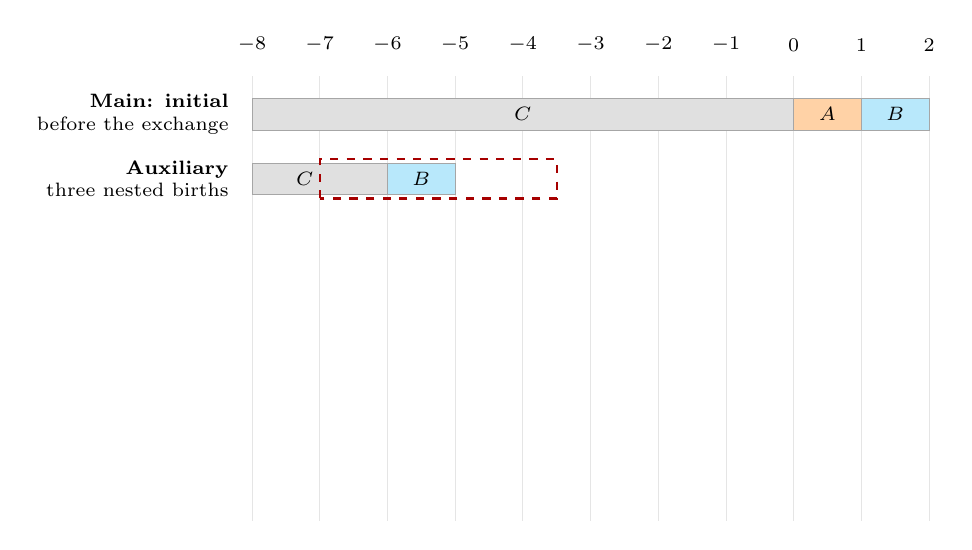
\begin{tikzpicture}[
  x=.86cm,y=1cm,
  bandA/.style={fill=orange!35,draw=black!35,line width=.3pt},
  bandB/.style={fill=cyan!28,draw=black!35,line width=.3pt},
  bandC/.style={fill=black!12,draw=black!35,line width=.3pt},
  lens/.style={draw=red!65!black,dashed,line width=.8pt}
]
  \foreach \geometrytick in {-8,-7,...,2} {
    \draw[black!10,line width=.3pt]
      (\geometrytick,.48) -- (\geometrytick,-5.17);
    \node[above,font=\scriptsize] at (\geometrytick,.67) {$\geometrytick$};
  }
  \geometryrow{0}{\textbf{Main: initial}\\before the exchange}
  \geometryband{0}{-8}{0}{C}
  \geometryband{0}{0}{1}{A}
  \geometryband{0}{1}{2}{B}
  \geometryrow{-.82}{\textbf{Auxiliary}\\three nested births}
  \geometrybandat{-.82}{-8}{-6}{C}{-7.22}
  \geometryband{-.82}{-6}{-5}{B}
  \draw[lens] (-7,-1.07) rectangle (-3.5,-.57);
\end{tikzpicture}

% the same coordinates, probed instead of drawn: x=.86cm must scale the abscissa and nothing else
\begin{tikzpicture}[x=.86cm,y=1cm]
  \pp{-8}{.48} \pp{-8}{-5.17} \pp{-8}{.67} \pp{2}{.67}
  \pp{-8.20}{0}
  \pp{-8}{-.20} \pp{0}{.20}
  \pp{0}{-.20} \pp{1}{.20}
  \pp{1}{-.20} \pp{2}{.20}
  \pp{-7}{-.82} \pp{-7.22}{-.82}
  \pp{-7}{-1.07} \pp{-3.5}{-.57}
\end{tikzpicture}

% \geometryband's midpoint is written as a braced pgfmath expression, ({(#2+#3)/2},#1): TeX's own
% answer for (-8+-6)/2 is what the canvas has to carry as an abscissa.
\pgfmathsetmacro{\bandmid}{(-8+-6)/2}
\pgfmathsetmacro{\bandedge}{(-8+0)/2}
\typeout{MID: (-8+-6)/2 = \bandmid, (-8+0)/2 = \bandedge}
\end{document}
